\section*{Suggested Reading:}
\begin{itemize}
  %\item Bias-Variance Tradeoff: UML 5.2
  \item CART Regression Trees ESL 9.2.2
  \item Pruning CART regression and regularization trees ESL 9.2
  \item $\ell_2$-regularized linear regression (Ridge regression): ESL 3.4.1,
    3.4.3, UML 13.1.1.
  \item $\ell_1$-regularized linear regression (Lasso): ESL 3.4.2, 3.4.3, UML
    25.1.3
  \item $\ell_1$-regularized logistic regression ESL 4.4.4
\end{itemize}


\section{Introduction}

Recall that we divided supervised learning into {\bf regression} problems 
(label set $\Y=\R$) and {\bf classification} problems (binary, where $\Y=\left\{ \pm 1
\right\}$ or multiclass, where $\Y=\left\{ 1,\ldots, k \right\}$).
\\~\\
So far in this course we've paid little attention to
{\bf regression} problems. We only saw linear regression.
\\~\\
So after talking a lot about classification, in this lecture we come back to
regression problems. As in the classification lecture, we will work on the
sample space $\X=\R^d$ - the $d$-dimensional Euclidean space, so that each
ssample is a feature vector with $d$ real entries. 
Many modern regression methods on $\X=\R^d$ use a principle called {\bf
Regularization}. 
\\~\\
So in this lecture we will introduce the concept of
{\bf regularization}, which is a fundamental concept in machine learning.
We will then see
four different modern regression methods, which are all different examples
of regularization. To keep classification in the picture, we will finish with a
classification method using regularization. 
%\\~\\
%Along the way we will discuss interesting topics such as
%the problem high-dimensional data $d\gg m$, sparsity, the problem of feature
%selection. The latter will lead us to next week's lecture on model selection and
% evaluation. 

\section{Regularization}


\subsection{The setup: Choosing $h\in\Hc$ by minimizing fidelity}

{\bf Regularization} is a principle that allows us to build a continuous family
of learners $\Ac_\lambda$, all producing hypotheses from a single
 hypothesis class $\Hc$.
\\~\\
 Let's think about general $\X$ and $\Y$ - so this section works for both
 regression and classification.
Assume that we have a learner $\Ac_0$ that chooses an hypothesis
$h_S\in\Hc$ 
from a given hypothesis class $\Hc$, based
on minimizing some cost function $\Fc_S(h)$ over $h\in\Hc$.
(Obviously, this cost function depends on the training sample
$S$.) 
This means that $h_S=\Ac_0(S)$ is given by
\[
  h_S := \text{argmin}_{h\in\Hc} \Fc_S(h)\,.
\]
~\\
The function $\Fc$ measures how well $h$ fits the training sample $S$. We can
call $\Fc(h)$ the {\bf fidelity term}.
\\~\\
We have seen a few examples for such learners already:
\begin{itemize}
  \item In linear regression, $\Fc_S(h)$ measures the {\bf sum of squares}
  \item In logistic regression, $-\Fc_S(h)$ is the {\bf likelihood} for the logistic
    regression model (which we want to
    maximize)
  \item In SVM, $-\Fc_S(h)$ is the {\bf margin} (which we want to maximize)
\end{itemize}
~\\
The best example for learners that minimize a cost function is
of course {\bf ERM}: In any learner based on {\bf Empirical Risk Minimization}, we
define some loss function $\ell(\cdot,\cdot)$ and 
define the empirical risk induced by $\ell$, with respect to the training sample
$S=\{\left( x_i,y_i \right)\}_{i=1}^m\subset (X\times \Y)^m$, to be
\[
  L_S(h) = \frac{1}{m} \sum_{i=1}^m \ell(h(x_i),y_i)\,.
\]
So an ERM learner fits in this framework if we take the fidelity term  
$\Fc_S(h)$ to be the empirical risk $L_S(h)$, and choose $h_S$ using
\[
  h_S = \text{argmin}_{h\in\Hc} L_S(h)\,.
\]

\subsection{Adding a regularization term}

If the hypothesis class $\Hc$ is ``too large'', we are concerned that minimizing
$\Fc_S$
over $\Hc$ may lead to over-fitting - namely, we are concerned our learner will
output 
 an hypothesis $h_S$ which will
not generalize well, because it's too well adapted to the particular training sample $S$.
\\~\\
One way to solve this problem would be to restrict $\Hc$. 
But a more elegant and flexible way is to leave $\Hc$ large, but change the learner
$\Ac_0$. We do this by changing the optimization problem that $\Ac_0$ uses to choose
$h_S$. Instead of 
\[
  h_S := \text{argmin}_{h\in\Hc} \Fc_S(h)\,.
\]
we choose $\lambda\geq 0$ and define the learner $\Ac_\lambda:S\mapsto h_S$ by
\[
  h_S := \text{argmin}_{h\in\Hc}\left[ \Fc_S(h)+  \lambda \Rc(h)\right] \,.
\]
~\\
The term $\Rc$ is called the {\bf regularization term}. The value $\Rc(h)$ will measure the
``complexity'' of the hypothesis $h$. The more complicated the hypothesis $h$,
the larger $\Rc(h)$ will be. 
\\~\\
So we see that in minimizing $ \Fc_S(h)+ \lambda \Rc(h)$ we now have a
{\bf tradeoff}:
\begin{itemize}
  \item On one hand, more complicated $h$, the better it can describe the
    training sample $S$, so the fidelity term $\Fc_S(h)$ will be smaller.
  \item On the other hand, the more complicated $h$, the larger $\Rc(h)$ will
    be. 
\end{itemize}

And conversely, the simpler $h$, the larger the fidelity term $\Fc_S(h)$ (as it
won't be able to describe the training sample very well) but the smaller
$\Rc(h)$ will be.
\\~\\
So $\lambda$ is a tradeoff parameter:
\begin{itemize}
  \item For $\lambda=0$, we have no regularization and are back to finding a
    minimizer of $\Fc_S(h)$.
  \item For $\lambda \to\infty$, the minimization problem pays no attention to
    the fidelity term and just wants to find the simplest possible $h\in\Hc$.
  \item Any finite value $\lambda\in(0,\infty)$ defines a specific tradeoff
    between the need for fidelity (small $\Fc_S(h)$) and the need for simplicity
    of $h$ (small $\Rc(h)$).
\end{itemize}
~\\
So, when we add regularization to the learner
$\Ac_0:S\mapsto\text{argmin}_{h\in\Hc} \Fc_S(h)$, we won't find a minimizer of
$\Fc_S(h)$ over $\Hc$. We are hoping that a minimizer of the regularized
objective function $\Fc_S(h)+ \lambda \Rc(h) $ (which does not minimize
$\Fc_S(h)$) will generalize better.
This is because, the larger the value of $\lambda$, the simpler this minimizer
will be.
~\\
We therefore get a {\bf family} of learners $\{\Ac_\lambda\}_{\lambda\in[0,\infty)}$. The
regularization parameter $\lambda$ controls the bias-variance tradeoff: for
$\lambda=0$ we get the most variance and least bias (most complicated $h$); for $\lambda\to\infty$ we
get the least variance and most bias (simplest $h$).
\\~\\
{\bf Example: Soft SVM}. We already saw one example for regularization - Soft
SVM. Recall that the Soft-SVM classifier classifies using the half-space $\VV{w}^\perp$
where $\VV{w}$ is a solution to the optimization problem

\begin{eqnarray*}
      & \text{minimize}   &  \lambda \norm {\VV{w}}^2 + \frac{1}{m}\sum_{i=1}^m
      \xi_i \\
      & \text{subject to} & y_i \cdot \left( \innerr{\VV{x}_i}{\VV{w}}
     +b \right) \geq 1-\xi_i  \,\,\text{and}\,\, \xi_i\geq 0 
    \end{eqnarray*}
~\\
    Here, the fidelity term is $\norm{\VV{w}}^2$. The smaller $\norm{\VV{w}}^2$,
    the better we fit the training data (in the sense of larger margin). 
    Indeed, we saw in the recitation that
    the total margin is proportional to $1/\norm{\VV{w}}$, so that minimizing  $\norm{\VV{w}}^2$
    means maximizing the margin. 
    The regularization term is  $\frac{1}{m}\sum_{i=1}^m \xi_i$. The smaller
    this term is, the ``simpler'' the hypothesis since we allow less violations
    of the margin\footnote{You'll note that here $\lambda$ is placed on the fidelity
    term, not on the regularization term. That happens sometimes. But in this
    lecture we'll use the structure $\Fc_S(h)+ \lambda \Rc(h) $ and put
  $\lambda$ in front of the regularization term.}.

    \subsection{Let's focus on Euclidean sample space, regression problems and
    ERM fidelity for the square loss}

    For most of this lecture, we'll focus on {\bf regression} problems on
    Euclidean sample space, so from now on, $\X=\R^d$ and
    $\Y=\R$. We'll focus on the most common fidelity term - the empirical risk
    $\Fc_S(h) = L_S(h)$. 
    Recall that the empirical risk $L_S$ is induced by a loss function
    $\ell(\cdot,\cdot)$. 
    When we talked about classification problems, most of the time we worked
    with the $0-1$ loss (the misclassification loss). In this lecture, when we
    talk about regression problems, we will work with the {\bf squared loss}
    $\ell(h(x),y)=(h(x)-y)^2$. So the empirical risk will be the sum of squares
    that we have seen when we talked about linear regression:
    \[
      L_S(h)= \sum_{i=1}^m \left( h(x_i)-y_i \right)^2\,.
    \]
~\\
    We will cover four modern regression methods - these will be the most advanced
    regression methods we will learn in this course. They are all based on
    adding a regularization term to ERM. The methods are:

    \begin{itemize}
  \item CART regression trees with pruning
  \item Linear regression with $\ell_0$ regularization, related to {\bf best subset selection}
  \item {\bf Ridge regression}: Linear regression with {\bf $\ell_2$ regularization}
  \item {\bf The Lasso}: Linear regression with {\bf $\ell_1$ regularization}
 \end{itemize}
~\\
    Near the end of the lecture we'll see a completely different example:
    $\ell_1$-regularized logistic regression. In that example, we will
    add a regularization term to fidelity based on  maximum likelihood  - not
    on ERM - in a classification problem. That will allow us to remember that
    the regularization principle is very general and not at all specific to
    regression, or to ERM fidelity. 

    \section{CART Regression Trees}

    Our first example for adding regularization to ERM is the CART algorithm for
    {\bf Regression Trees}. We have only seen CART classification trees, so before we
    get to adding regularization, let's
    start by defining a regression tree and see that we already understand the
    CART algorithm for fitting a regression tree.
\\~\\
     This section assumes you and understand classification (decision)
    trees, and the CART algorithm for growing a classification tree. If you
    don't, it is recommended that you review the classification lecture handout. 
   

    

    \subsection{Regression Trees}

    For a Tree Partition $\reals^d=\biguplus_{j=1}^N B_j$ of
     $\reals^d$ into $N$ axis-parallel boxes, and label assignments $c_j \in \R$
     ($j=1,\ldots, N$) assigning label $c_j\in \R$ to box $B_j$, the
     regression tree $h\in\Hc_{RT}$ is a function
     $h:\reals^d\to\R$
      defined by 
     \[
       h(\VV{x}) = \sum_{j=1}^N c_j \mathbf{1}_{B_j}(\VV{x})
     \]
     where $\mathbf{1}_{B_j}$ is the indicator function of $B_j$. 
\\~\\
  The only difference from a classification tree is that now the labels $c_j$
  are real numbers, not classes in $\left\{ \pm 1 \right\}$. 
  Any function in this hypothesis class corresponds to a decision tree leading
  to a {\bf numerical} decision. 

    \subsection{Growing a CART regression tree}

    As for classification trees, given a training sample $S$,
     we would ideally like to search $\Hc_{RT}$ for a tree minimizing the
     empirical risk - namely, to learn using the ERM principle. But as for
     classification trees, this is computationally hard, so must use a heuristic
     to choose the tree based on the training sample.
\\~\\
     Suppose that we have already somehow 
 decided to use a certain Tree Partition of $\reals^d$ that consists of $N$ disjoint boxes,
 $\reals^d=\biguplus_{j=1}^N B_j$. Let $S=\left\{ (\VV{x}_i,y_i)
 \right\}_{i=1}^m$, where $\VV{x}_i\in \R^d$ and $y_i\in\R$ be our training sample.
\\~\\
 {\bf Exercise.} Let $y_1,\ldots,y_k\in\R$ be real numbers. Then
 \[
   \argmin_{c\in\R} \sum_{i=1}^k (y_i-c)^2
 \]
 is simply the sample average
 \[
   ave(y_1,\ldots,y_k) = \overline{y} = \frac{1}{k}\sum_{i=1}^m y_i\,.
 \]
~\\
 This means that given an existing tree partition, the empirical risk would be
 minimized by choosing the label $c_j:= ave(y_i \,|\, y_i\in B_j)$, namely, the
 average of the labels of the training samples in $B_j$.
\\~\\
 The CART heuristic for growing a regression tree starts with $B_0=\R^d$ and recursively splits each existing
 box $B$ as follows:
 \begin{itemize}
  \item for each coordinate $i\in\left\{ 1,\ldots d \right\}$, and each
    potential chopping value $t\in\reals$, let $g_i(t)$ be the 
    the lowest empirical misclassification risk (with respect to the training
    sample $S$) incurred by
      chopping the box $B$ at value $t$ along coordinate $i$.
      Calculate the value $g_i(t)$ for each $i$ and $t$ as follows: 
    \begin{itemize}
      \item For each $t\in\reals$ (such that $t$ is a valid chopping point for
	$B$ along coordinate $i$) let 
	$B_{+,t} := \left\{ \VV{x}\in\reals\,|\, x_{i}>t \right\}$ 
	and 
	$B_{-,t} := \left\{ \VV{x}\in\reals\,|\, x_{i}\leq t \right\}$ 
	by the two boxes obtained from $B$ by chopping the box $B$ along
	coordinate $i$ at the value $t$. 
      \item Now let $\hat{y}_S(B_{\pm,t})$ be the class assignment
	for box $B_{\pm,t}$ that minimizes the empirical  risk for square loss (with respect to
        training sample $S$). Namely, $\hat{y}_S(B_{+,t})=
        ave(y_i\,|\, y_i\in B_{+,t})$ and similarly 
        $\hat{y}_S(B_{-,t})=
        ave(y_i\,|\, y_i\in B_{-,t})$. Now 
      let
        $L^S_{\hat{y}_S(B_{\pm,t})}$ be that optimal empirical
        risk for square loss incurred by these class assignments.
    \item Now, let $g_i(t) = L^S_{\hat{y}_S(B_{+,t})} +
      L^S_{\hat{y}_S(B_{-,t})}$. Convince yourself that this is
      the best empirical risk that can be incurred when
      chopping the box $B$ at value $t$ along coordinate $i$. 
      A simple formula for $g_i(t)$ is 
      \[
        g_i(t) = \sum_{i:\V{x}_i\in B_{+,t}} (y_i-\hat{y}_S(B_{+,t}))^2 
        + \sum_{i:\V{x}_i\in B_{-,t}} (y_i-\hat{y}_S(B_{-,t}))^2  \,.
      \]
    \end{itemize}

  \item Let $t_i := argmin_{t\in\reals}\,\, g_i(t)$ be the {\bf best} chopping point along
    coordinate $i$. Calculate $t_i$ for each coordinate $i=1,\ldots d$.
  \item Let $i_* := \argmin_{1\leq i \leq d} g_i(t_i)$ be the {\bf best} coordinate along which to chop $B$.
  \item Now chop $B$ along coordinate $i_*$ at the value $t_{i_*}$.
\end{itemize}
~\\
We continue chopping each box into two boxes unless:
\begin{itemize}
  \item The box is at the maximal depth specified, or
  \item The number of training samples in the box is smaller than the minimal
    number specified.
\end{itemize}
~\\
So the CART algorithm for growing a regression tree (when using the square loss)
is exactly the same as the
algorithm for growing a classification tree, just using averages instead of
majority votes for the labels.


    \subsection{Pruning a CART regression tree - using regularization}

    We finally get to our first regularization example. 
\\~\\
    The CART algorithm for growing a regression tree results in a mostly balanced
    tree. As we mentioned in the classification lecture, we may have done too
    many splits. Each split we do decreases the bias (as we have a more
    complicated hypothesis, with more expressive power) but also increases the
    variance (as the labels for prediction in the leaf are averaged over fewer
    training samples).
\\~\\
    The last stage of CART (for both regression and classification trees, but
    let's talk about regression trees now) is  {\bf pruning} the grown tree.
    (To Prune in English means to cut off some branches off a tree.)
    In the context of regression and classification trees, this
    means decreasing the tree size by merging together some boxes
    we've chopped in the growing stage - to reach a better bias-variance
    tradeoff that will lead to better generalization. 
    \\~\\
    Consider a training
    sample $S$ and a  regression tree
    $T$ induced by a
    partition $\reals^d=\biguplus_{j=1}^N B_j$. 
%
The empirical risk (for
    square loss) of $T$ on $S$ is 
    \[
      L_S(T) = \sum_{j=1}^N \,\,\sum_{i\,:\, \V{x}_i\in B_j}
      (y_i-\hat{y}_S(B_j))^2\,.
    \]
    This will be our fidelity term $\Fc_S(T)$.
    \\~\\
    Now let $T_0$ be the fully grown tree obtained from the growing stage of
    CART. 
    Let's write $T\subset T_0$ if the tree $T$ is a sub-tree of $T_0$, namely,
    if $T$ is obtained from $T_0$ by merging some boxes of $T_0$.
\\~\\
For our regularization term we simply use $\Rc(T)=|T|$, where $|T|$ denotes the
number of leaves (boxes) of $T$ - the same quantity we denoted above by $N$.
This is a good
    measure for complexity of an hypothesis in $\Hc_{RT}$: more leaves is 
    a more complicated tree, since it uses
    a finer partition of $\R^d$ into boxes.
\\~\\
    Our regularization problem will be
    \begin{eqnarray} \label{T}
      \min_{T\subset T_0} \left[L_S(T) + \lambda\cdot |T|\right]\,.
    \end{eqnarray}
~\\
Namely among all the subtrees of our fully grown $T_0$, we look for the
      one optimally balancing empirical risk and hypothesis complexity.
\\~\\
Note that we do {\bf not} optimize this objective over the entire hypothesis
      class $\Hc_{RT}$ (that would be infeasible) - just over subtrees of the large tree we grew by the CART 
      greedy splitting. 
\\~\\
      {\bf Is there an efficient implementation?} Yes. It turns out that there
      is a simple, efficient algorithm for solving the minimization problem
      \eqref{T} - see ESL 9.9.2 for details. 

    \subsection{The complete Random Forest algorithms for regression and for
    classification}

    Finally we know all the details  of random forests - for both regression and
    classification. A single tree is grown using a heuristic (such as CART) that
    consists of two stages - growing a full tree, then pruning that tree. A
    single tree needs three tuning parameters - the maximum number of levels,
    the minimum number of training samples in a leaf (a box), and the
    regularization parameter $\lambda$. When we run bagging on top of the CART
    algorithm, with the de-correlation trick (restricting each split to a random
    subset of coordinates), we get a random forest - either for regression or
    classification. In a typical random forest implementation there is no
    pruning - it is too computationally expensive to solve the pruning 
    problem \eqref{T} for each tree if we're training hundreds of trees or more.
\\~\\
    We've seen trees and forests over three lectures - and finally we know
everything we need to know about them.


\section{Modern Regression methods on $\R^d$}


    \subsection{Linear Regression with high-dimensional data}

    We now turn to modern regression methods based on the linear hypothesis
    class - with regularization. Recall that the first hypothesis class we saw
    in this course was the hypothesis class of linear functions for regression: 
     \[
 \Hc_{lin} = \left\{h: \quad h(x_1,\ldots,x_d)= w_0 + \sum_{i=1}^d x_i w_i,  \quad w_0,w_1,\ldots, w_d\in\R
 \right\}
    \]
~\\
    When we introduced linear regression we assumed that the training sample
    size $m$ was not smaller than the number of features $d$: we assumed $m\geq
    d$. We saw that we prefer $m\gg d$, since if $m\sim d$ the variance of the
    linear hypothesis we find by least squares (the learning algorithm we
      derived both as ERM for the square loss and using the maximum likelihood
    principle for Gaussian noisy label) can be large.
\\~\\
    But in modern learning problems based on $d$ features (namely, on the sample
    space $\X=\R^d$) very often $d$ can be quite large. Linear regression was
    invented when features were measured and recorded manually.  In the last few
    decades it became very easy to
    collect features and record them automatically, and a typical regression
    problem can easily have $d\sim m$ or even $d\gg m$. 
\\~\\
    When $d\sim m$ or, worse, $d\gg m$, we will have correlated features. The
    coefficients fitted by linear regression will be poorly determined - for
    example, a large positive coefficient for some feature can be cancelled out
    by a large negative coefficient for an almost-parallel feature. 
    So the linear regression learner we saw should not be used for $m\sim d$ and
    cannot be used for $d>m$.

    \subsection{Best subset selection}

    Recall that each hypothesis in $\Hc_{lin}$ corresponds to a unique weight
    vector $\V{w}\in\R^{d}$, where $\V{w}=(w_1,\ldots,w_d)$, with an intercept
    $w_0\in\R$. {\bf Unlike the linear regression class, we won't include $w_0$
    inside the vector $\V{w}$}, so that $\V{w}\in\R^d$.
   \\~\\ 
    Recall our $d$-by-$m$ regression matrix $X$ (now we don't have $"1"$ entries in the first
row), and vector $\V{y}$, and recall that we can write
\[
  L_S(\V{w}) = \norm{ w_0\mathbf{1} + X^\Tr\V{w} -\V{y}}^2
\]
for the empirical risk (for square loss), where $\mathbf{1}$ is a vector whose entries are all $1$. 
\\~\\
    The ultimate solution to the issues of linear regression on large $d$
    is known as {\bf best subset selection}:
\begin{eqnarray*}
  & \text{minimize}_{w_0\in\R,\V{w}\in\R^{d}}   &  \norm{  w_0\mathbf{1} + X^\Tr\V{w} -\V{y}  }^2 \\
      & \text{subject to} &  \norm{\V{w}}_0 \leq t
    \end{eqnarray*}
    Where $\norm{\V{v}}_0 = \#\left\{ i\,|\, v_i\neq 0 \right\}$. 
    (Note that the ``norm'' $\ell_0$ is not really a norm (why?).)
\\~\\
This is perfect! We specify $t$ and among all subsets $t$ features out of the $d$
features in our training sample, we find the one with lowest training loss (in the sense of
least squares). Now we just play with $t$ to walk on the bias-variance tradeoff
- on one hand we would like $t$ to be large enough to have low bias (descriptive
power) and one the other hand we would like $t$ to be small enough (e.g. much smaller than
$m$) so we will avoid all the nasty effects of large $d$ mentioned above. 
~\\ The bad news? You won't be surprised to hear that this problem is known to
be NP-hard. Indeed the quantity $\norm{\V{w}}_0$ is not convex, and solving this
smells like a combinatorial search over all possible subsets of size $t$.
\\~\\
What can we do?
Instead of 
\begin{eqnarray*}
  & \text{minimize}_{w_0\in\R,\V{w}\in\R^{d}}   &  \norm{  w_0\mathbf{1} + X^\Tr\V{w} -\V{y}  }^2 \\
      & \text{subject to} &  \norm{\V{w}}_0 \leq t
    \end{eqnarray*}
    we will want to consider some other constrain on the coefficient vector
    $\V{w}$ that will measure its complexity. For a norm $\norm{\cdot}$ on
    $\R^d$, we'll consider instead 
    \begin{eqnarray*}
  & \text{minimize}_{w_0\in\R,\V{w}\in\R^{d}}   &  \norm{  w_0\mathbf{1} + X^\Tr\V{w} -\V{y}  }^2 \\
      & \text{subject to} &  \norm{\V{w}} \leq t
    \end{eqnarray*}
~\\
    It is simpler to consider an {\bf unconstrained}  form of these optimization
    problems - instead of specifying the constrain $t$, we'll specify a
    regularization parameter $\lambda$ and consider
\[
     \text{argmin}_{w_0\in\R,\V{w}\in\R^{d}} \left[L_S(w_0,\V{w})+  \lambda
     \norm{\V{w}} \right]
\]


    So this is where regularization comes in.
\\~\\
        The following three regression methods all choose a linear hypothesis in
    $\Hc_{lin}$ using
\[
  \text{argmin}_{w_0\in\R,\V{w}\in\R^{d}} \left[L_S(w_0,\V{w})+  \lambda
  \Rc(\V{w}) \right]
\]
where the fidelity term is just the empirical risk (sum of squares)
\[
  L_S(w_0,\V{w}) = \sum_{i=1}^m \left( w_0 + \innerr{\V{w}}{\V{x}_i} -y_i \right)^2\,.
\]
The regularization term measures the complexity of the linear hypothesis $\V{w}$. 
\\~\\
We will explore three different regularization terms, based on three different
norms. For a vector $\V{v}\in\R^d$, with $\V{v}=(v_1,\ldots,v_d)$ 
define the following norms:

\begin{itemize}
  \item The $\ell_2$ norm: $\norm{\V{v}}_2 = \sqrt{\sum_{j=1}^d |v_i|^2}$ (our
    usual Euclidean norm)
  \item The $\ell_1$ norm: $\norm{\V{v}}_1 = \sum_{j=1}^d |v_i|$
  \item The $\ell_0$ ``norm'':  $\norm{\V{v}}_0 = \#\left\{ i\,|\, v_i\neq 0
    \right\}$. (Again, this is not actually a norm.)
\end{itemize}


We'll define three corresponding regression learning algorithms that learn $h\in\Hc_{lin}$:
\begin{itemize}
    \item The learner 
    \[
      \text{argmin}_{w_0\in\R,\V{w}\in\R^{d}} \norm{ w_0\mathbf{1} + X^\Tr\V{w} -\V{y}  }^2
+  \lambda \norm{\V{w}}^2_2
    \]
    is called {\bf Ridge Regression} or {\bf $\ell_2$-regularized linear
    regression}.
 \item The learner 
    \[
      \text{argmin}_{w_0\in\R,\V{w}\in\R^{d}} \norm{  w_0\mathbf{1} + X^\Tr\V{w} -\V{y}  }^2
+  \lambda \norm{\V{w}}_1
    \]
    is called {\bf Lasso} or {\bf $\ell_1$-regularized linear
    regression}.
  \item The learner 
    \[
      \text{argmin}_{w_0\in\R,\V{w}\in\R^{d}} \norm{  w_0\mathbf{1} + X^\Tr\V{w} -\V{y}  }^2
+  \lambda \norm{\V{w}}_0
    \]
    is related to {\bf best subset regression}, and is sometimes called by 
    that name.
\end{itemize}
~\\
(There is an important detail regarding intercept: see below.)
\\~\\
For all three, if $\lambda=0$ we get our usual linear regression. 
For all three, as $\lambda \to \infty$ we get $\hat{\V{w}}\to 0$ so the
regression fits an intercept only (a constant function). 
But they are very very different from one another. 

\subsection{$\ell_0$ regularization: Best subset selection}

The first regularization we will explore uses $\Rc(\V{w}) = \norm{\V{w}}_0$.
\\~\\
The problem
 \[
      \text{argmin}_{w_0\in\R,\V{w}\in\R^{d}} \norm{  w_0\mathbf{1} + X^\Tr\V{w} -\V{y}  }^2
+  \lambda \norm{\V{w}}_0
    \]
is related (but not equivalent) to the subset selection problem we mentioned above.
\\~\\
Here we have a tradeoff between the sum of
squares $L_S(\V{w})$ and the number of features used $\norm{\V{w}}_0$. At
certain critical values of $\lambda$, as $\lambda$ grows, less and less
features will be allowed, until at some large value of $\lambda$ we are left
with $\V{w}=0$ so we only have  the intercept left. (Note that we are not
including the intercept in the regularization term.) 
%
% future classes - review lagrange form and convert between the two forms 
%
\\~\\
Note that while this problem is NP hard, there are still software packages that
solve it for small $d$. So if you have $d\approx 40$ you may still use best
subset selection. 

\subsection{Ridge}

Ridge regression is a nickname for linear regression with the regularization term
$\Rc(\V{w})=\norm{\V{w}}_2^2$:

\[
      \text{argmin}_{w_0\in\R,\V{w}\in\R^{d}} \norm{ w_0\mathbf{1} + X^\Tr\V{w} -\V{y}  }^2
+  \lambda \norm{\V{w}}^2_2
    \]
    Observe that this is a convex optimization problem, indeed a quadratic
    program. 
\\~\\
Ridge typically shrinks shrinks the regression coefficients:
    \begin{figure}[h!]
      \centering
      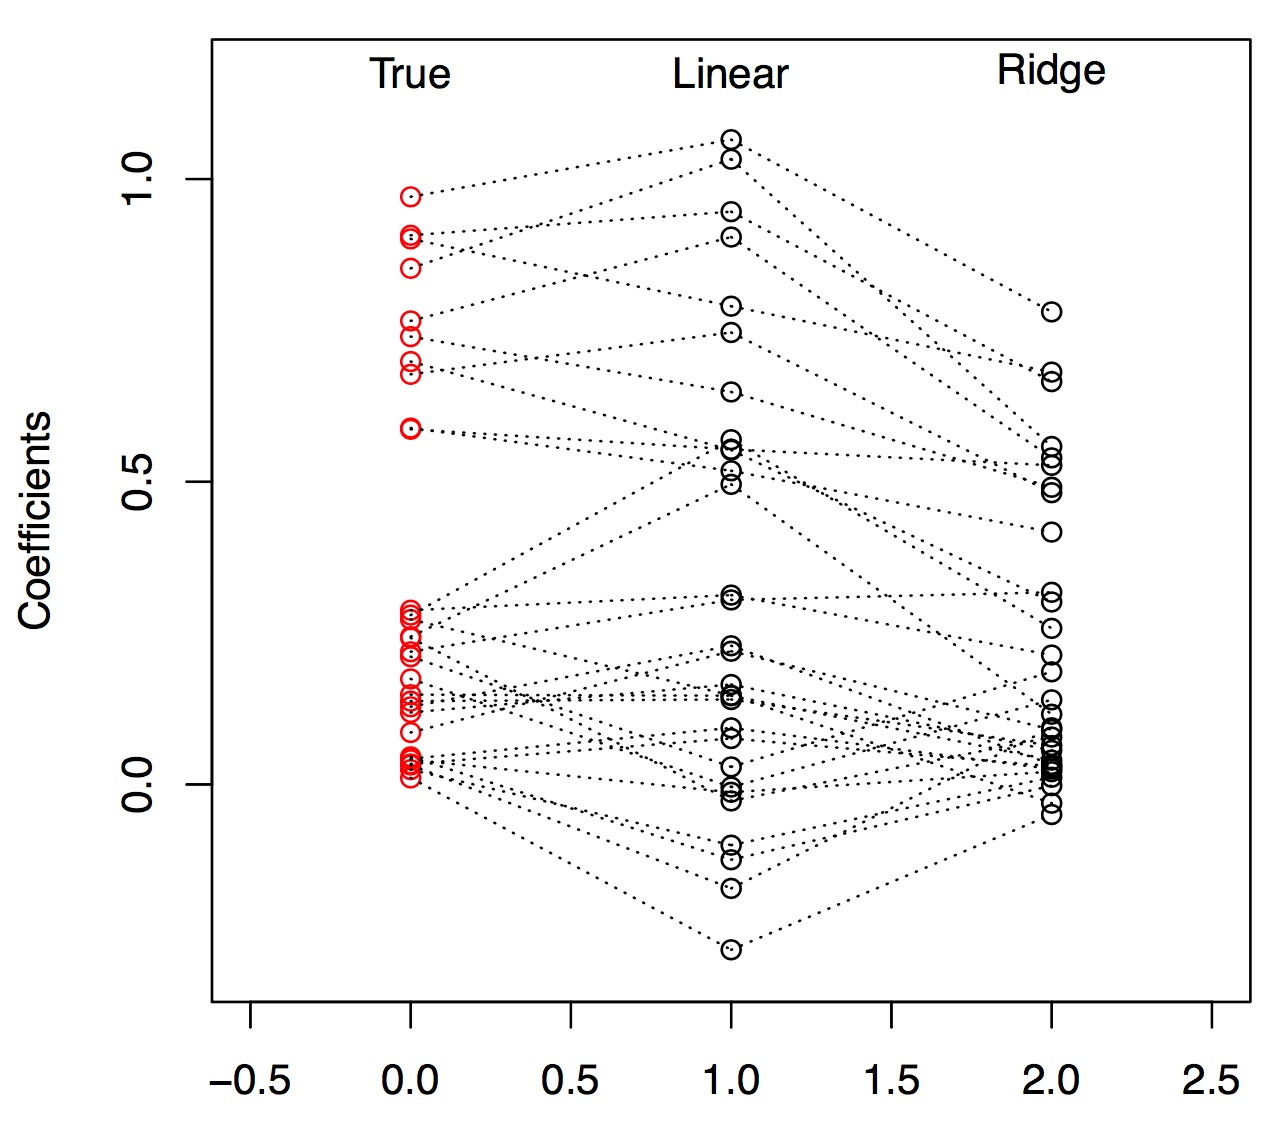
\includegraphics[width=3in]{ridge_coefs.jpeg}
      \caption{Left to right:
        Original weights $\V{w}$ in a linear model $\V{y}=X^\Tr
        \V{w} + noise$, weights fitted by linear regression ($\lambda=0$),
      weights fitted by Ridge ($\lambda>0$). Source: Ryan Tibshirani Data Mining slides, CMU 36-462/36-662 }
    \end{figure}
~\\
Denote by $\hat{\V{w}}_\lambda^{ridge}$ the
minimizer of the ridge problem. For $\lambda=0$ we get the least squares
(standard linear regression solution) and  for $\lambda\to\infty$ we get 
$\hat{\V{w}}_\lambda^{ridge}\to0$. As $\lambda$ increases, bias  increases and
variance decreases. 
\\~\\
How do we do find the Ridge solution computationally?
There is actually no need to use a QP solver: ridge is the only case in this
course (other than standard linear regression) where we have a 
{\bf closed-form}
solution for the minimizer. Applying the same method we used in linear
regression (calculating the gradient with respect to $\V{w}$ and looking for an
extremal point) we find that 
  \[
    \frac{\partial}
    {\partial w_i}
    \left[
    \norm{ w_0\mathbf{1} + X^\Tr\V{w} -\V{y}  }^2
  +  \lambda \norm{\V{w}}^2_2 \right]=0 \qquad i=1,\ldots,d
  \]
leads to the linear system
\[
  X\V{y} = (XX^\Tr+\lambda I)\V{w} \,.
\]
Observe that for $\lambda=0$ we recover the normal equations for linear
regression. The value of regularization is now clear - even if $XX^\Tr$ is not
invertible, even for $d>m$, for any $\lambda>0$ we always have that
$(XX^\Tr+\lambda I)$ is invertible. 
\\~\\
The SVD method for calculating the linear regression weights generalizes to
Ridge regression. Let $X=U\Sigma V^\Tr$ be an SVD of $X$, with singular values
$\{\sigma_i\}$. In the recitation you will prove that  the Ridge solution is
given by 
\[
  \hat{\V{w}}_\lambda^{ridge} = U \Sigma^\lambda V^\Tr\V{y}
\]
where $\Sigma^\lambda$ is diagonal whose $(i,i)$ entry is 
\[
  \frac{\sigma_i}{\sigma_i^2+\lambda}\,.
\]
~\\
The regularization parameter $\lambda$ controls the bias-variance tradeoff.
Here's an example: 

\begin{figure}[H]
      \centering
      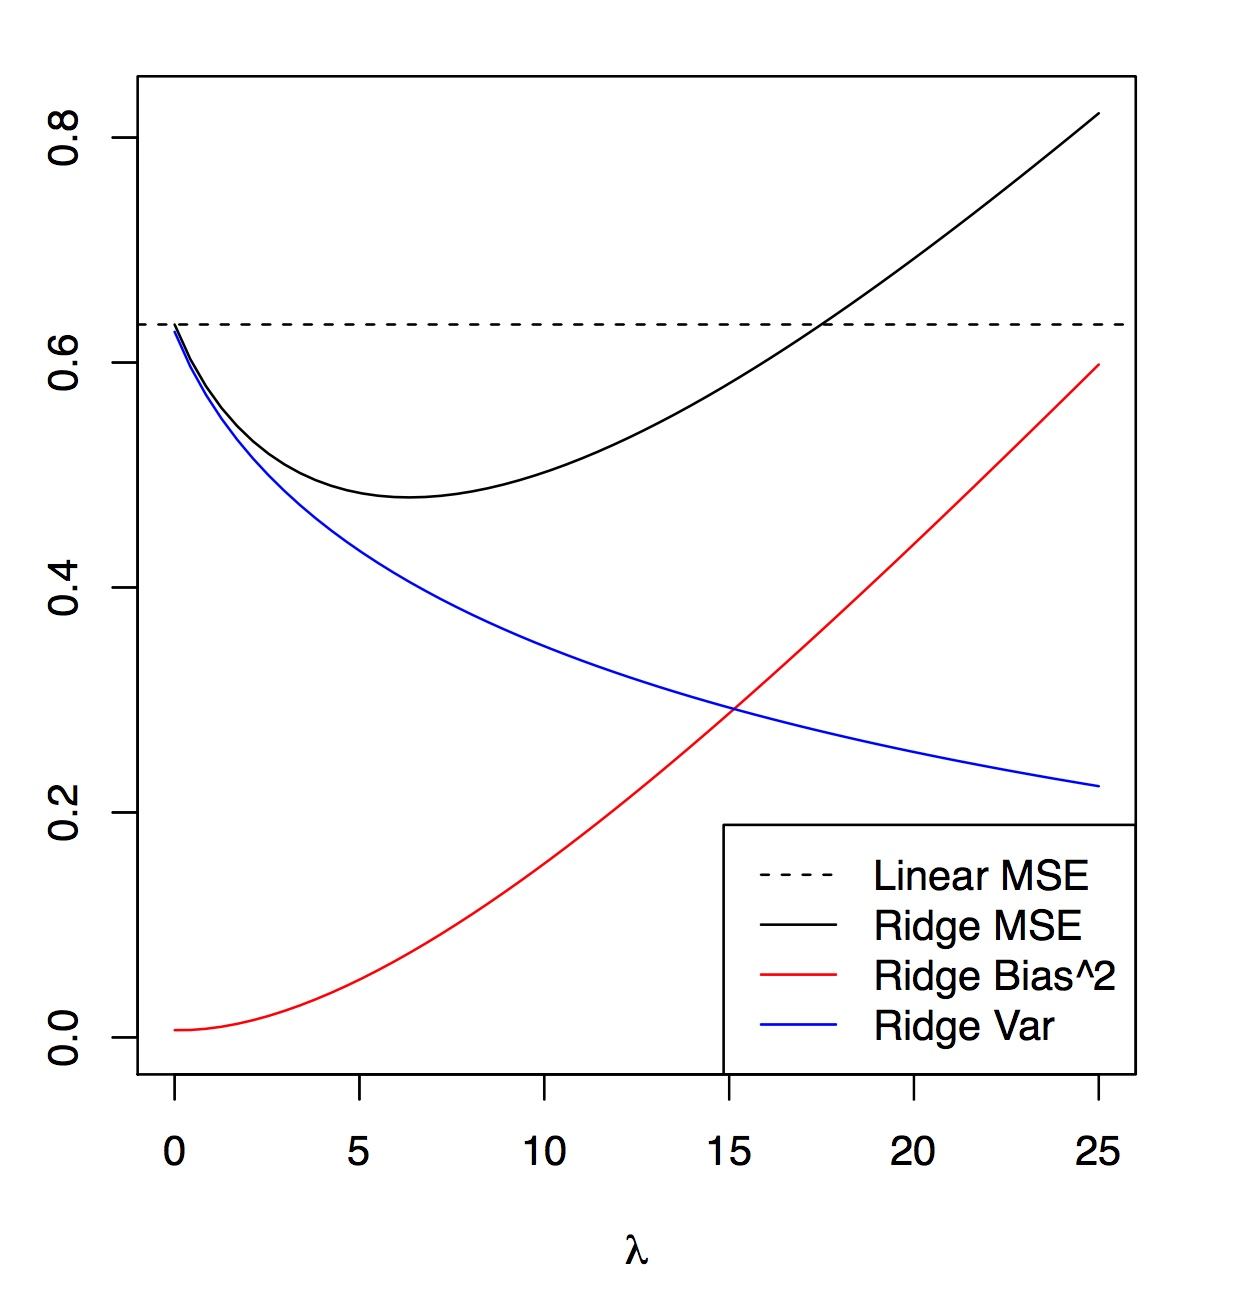
\includegraphics[width=3in]{ridge_bias_variance.jpeg}
      \caption{Bias, variance and MSE (mean square error) of a regression
      problem using Ridge regression, over $\lambda$. Source: Ryan Tibshirani Data Mining slides, CMU 36-462/36-662 }
    \end{figure}

\paragraph{Regularization Path.}
It is interesting to trace each individual weight $(\hat{w})_i$ for $1\leq i\leq
d$ as $\lambda$ changes. Such a plot is called the {\bf Regularization Path} of
the particular problem at hand. Observe how the weights start from the linear
regression weights (for $\lambda=0$) and follow a decay that looks roughly like
$1/\lambda$ decay as $\lambda$
grows. 

\begin{figure}[H]
      \centering
      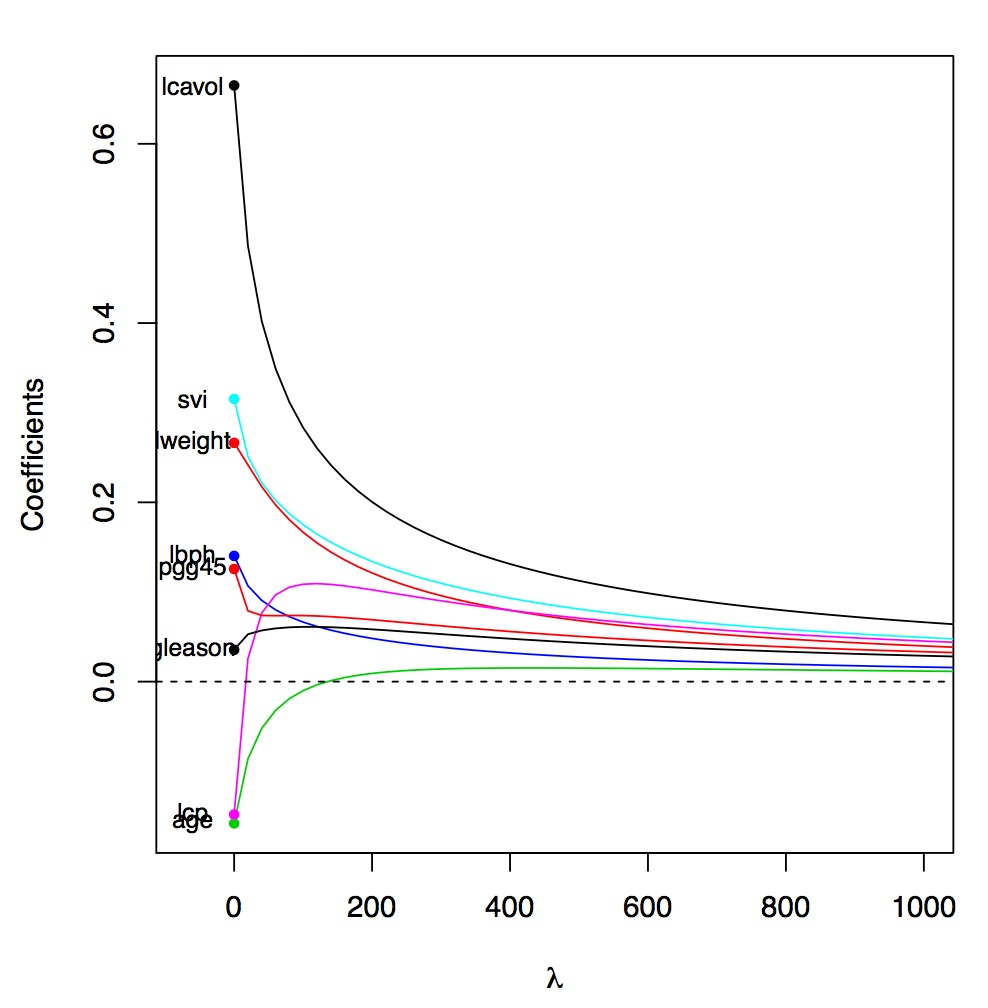
\includegraphics[width=3in]{ridge_path.jpeg}
      \caption{Regularization Path of a Ridge regression, over $\lambda$.
      Source: Ryan Tibshirani Data Mining slides, CMU 36-462/36-662 }
    \end{figure}


\subsection{Lasso}


So Ridge regression is a good method for using linear regression when $d$ is large or,
when $d>m$, or when
$XX^\Tr$ is not invertible. It's also a good way to get a simple handle on the
bias-variance tradeoff of linear regression. But is does not do what best-subset
can do, namely, {\bf select}
a specific subset of the features / variables  to use for regression.
\\~\\
{\bf The Lasso}\footnote{The name is an acronym for {\bf Least Absolute
  Shrinkage and Selection Operator}, but
you might as well think about the Lasso that cowboys (and Wonder Woman) use.}  is a nickname for $\ell_1$ regularized linear regression:
\[
      \text{argmin}_{w_0\in\R,\V{w}\in\R^{d}} \norm{ w_0\mathbf{1} + X^\Tr\V{w} -\V{y}  }^2
      +  \lambda \norm{\V{w}}_1\,.
    \]
    Observe that this is a convex optimization problem, indeed a quadratic
    program.
\\~\\
This is 
one of the most effective and well known methods for modern regression. 

\begin{figure}[H]
      \centering
      
\includegraphics[width=3in]{lasso_rope.jpg}
      \caption{A Lasso}
    \end{figure}
~\\
    It has the same behavior as Ridge for $\lambda=0$ and $\lambda\to\infty$,
    but in between, it is completely different. Lasso solutions - the weight
    vectors $\hat{\V{w}}_\lambda^{lasso}$ produced by Lasso -  are {\bf
    sparse}, meaning that they have few nonzero entries. 
    The larger $\lambda$, typically the more zeros $\hat{\V{w}}_\lambda^{lasso}$
    will have - so it gets sparser and sparser until, in the limit
    $\lambda\to\infty$, it is the zero vector. 
    Let's compare Ridge and Lasso coefficients:
    

        \begin{figure}[H]
      \centering
      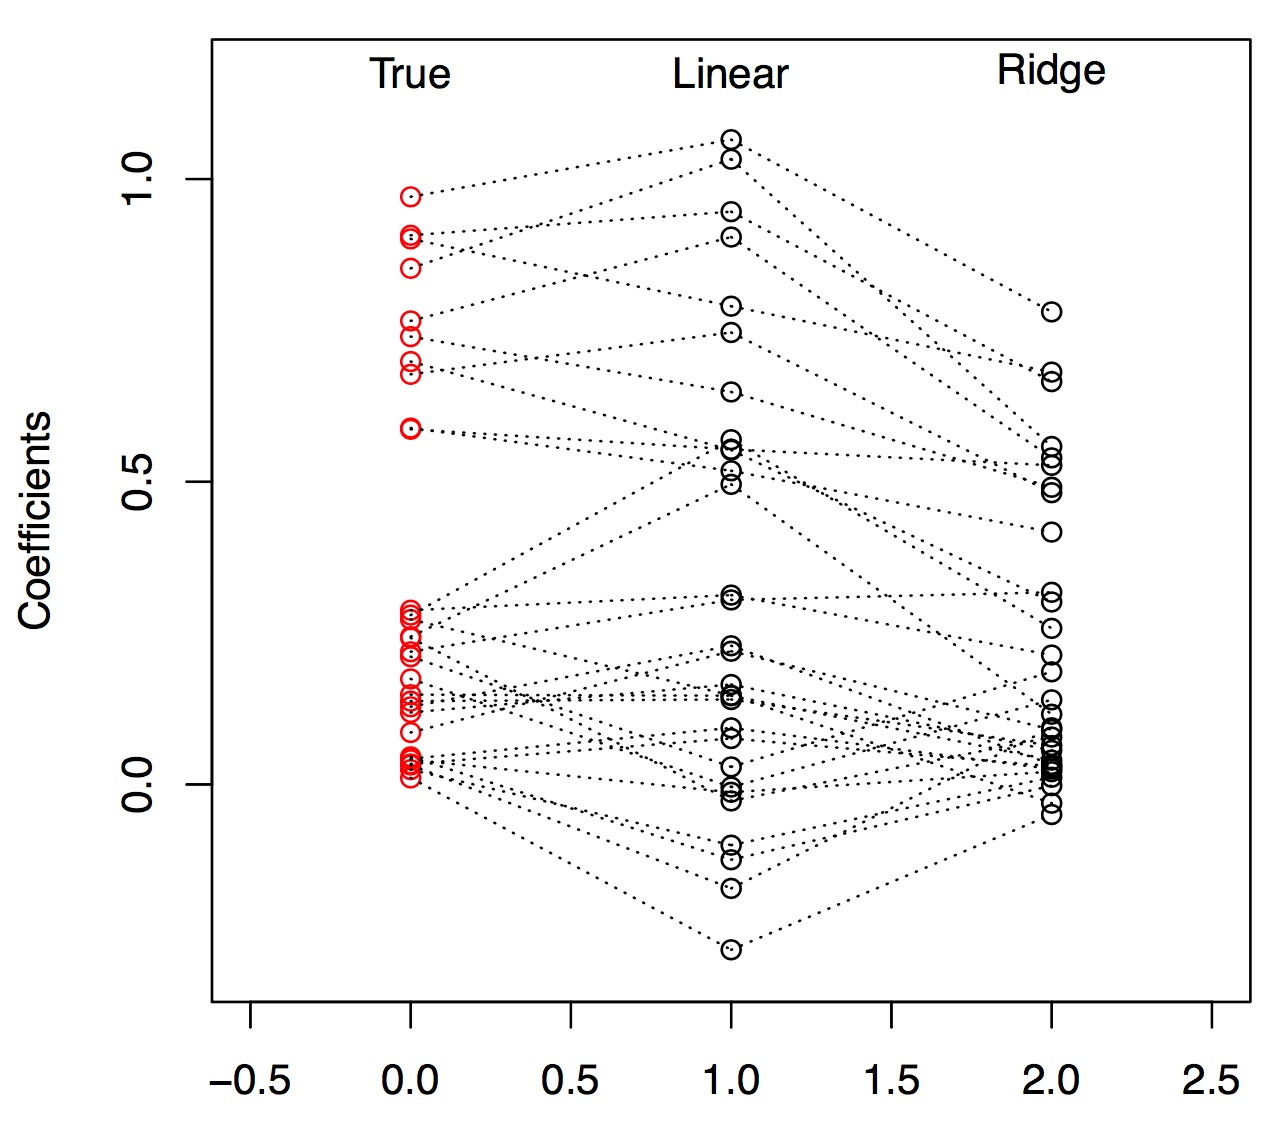
\includegraphics[width=3in]{ridge_coefs.jpeg}
      \,\,
      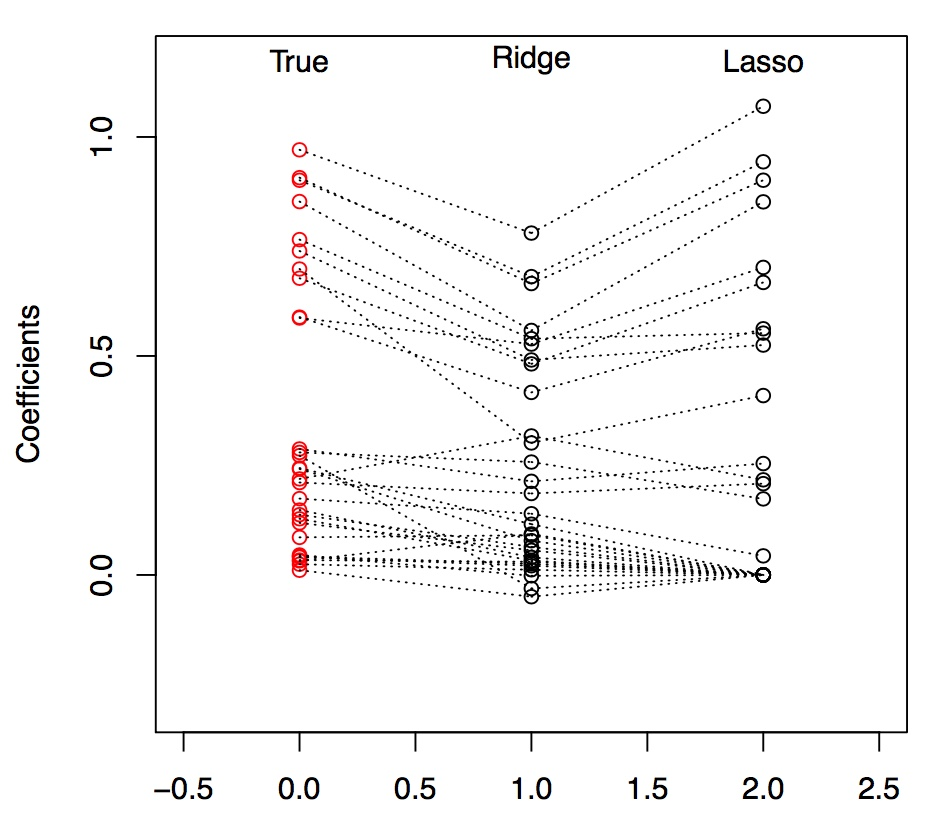
\includegraphics[width=3in]{lasso_coefs.jpeg}
      \caption{Right: Ridge weights. 
        Left: Lasso weights on the same problem. Note how in Lasso, many
        coefficients are sent to $0$, so that the weight vector is {\bf sparse.}
        Source: Ryan Tibshirani Data Mining slides, CMU 36-462/36-662 }
    \end{figure}
~\\
Let's also compare the Regularization Path or Ridge and Lasso:
\begin{figure}[H]
      \centering
      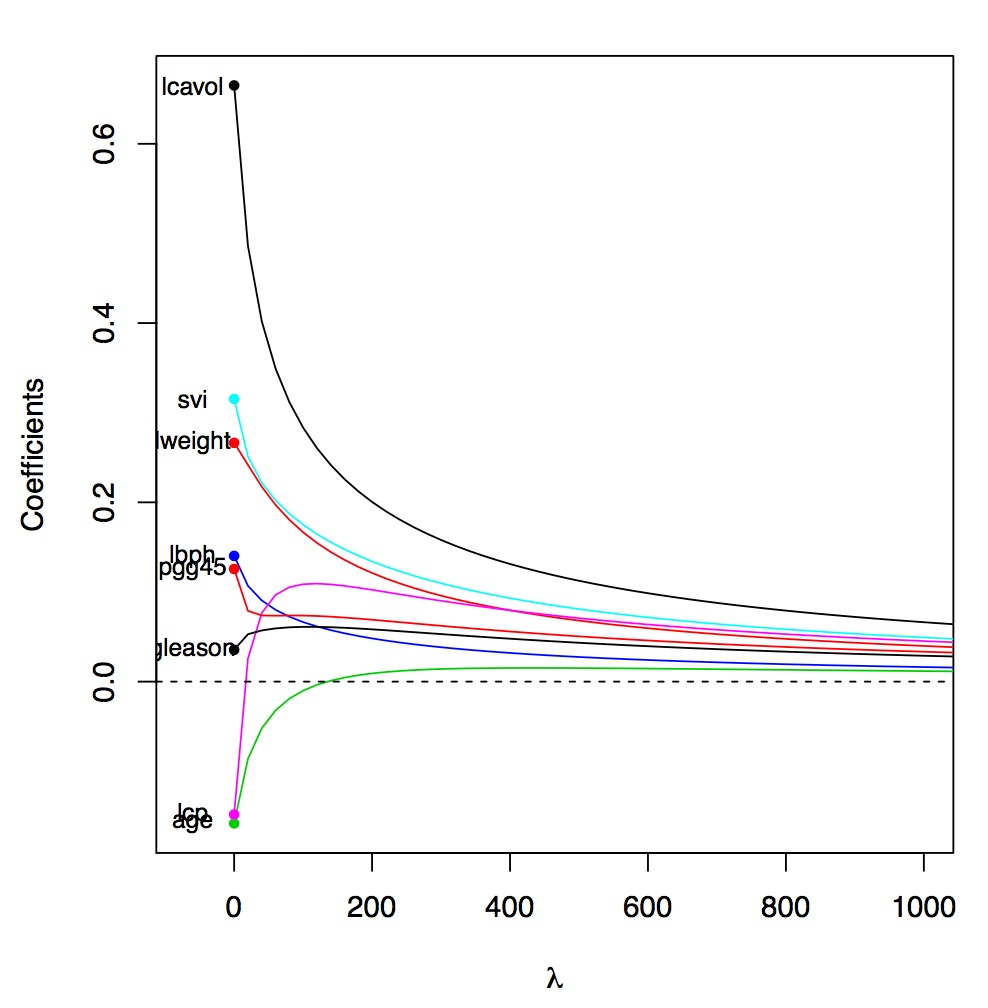
\includegraphics[width=3in]{ridge_path.jpeg}
      \,\,
      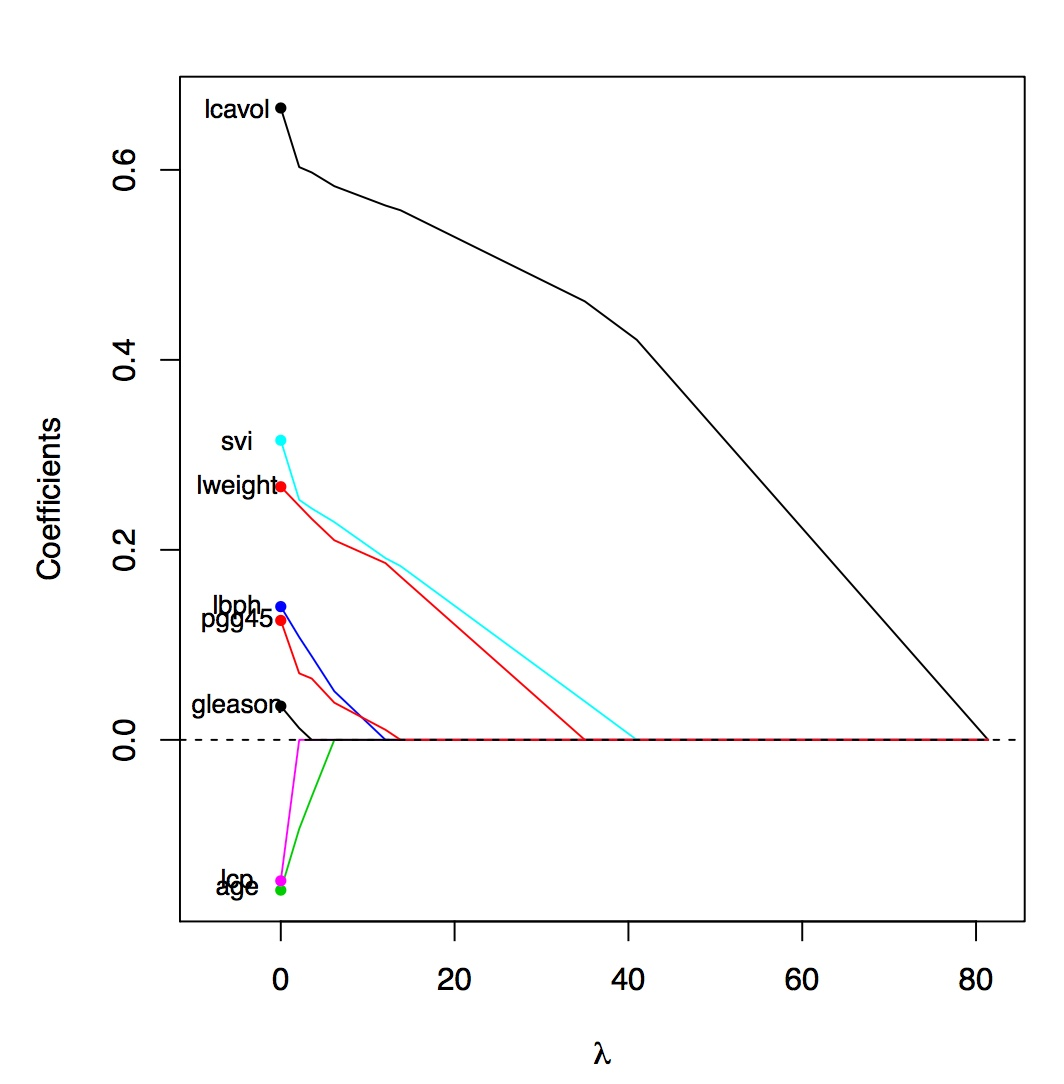
\includegraphics[width=3in]{lasso_path.jpeg}
      \caption{Right: Ridge regularization path. 
        Left: Lasso regularization path on the same problem. 
        Note how in Lasso, many
        coefficients are sent to $0$, so that the weight vector is {\bf sparse.}
        Source: Ryan Tibshirani Data Mining slides, CMU 36-462/36-662 }
    \end{figure}


\paragraph{Computational considerations.}
The Lasso is a convex optimization problem, indeed a quadratic program. There
are specialized solvers for the Lasso, which calculate the entire regularization
path (namely, solve the problem for all values of $\lambda$ at once) at the same
computational cost as solving Ridge. 

\paragraph{The Lasso is a kind of subset selection.}

For each value of $\lambda$, the Lasso solution has certain weights set to zero
and others nonzero. Looking at the ``active set'' - the features with nonzero
weights at the Lasso solution - is a way to know which features / variables are
important for the regression. The larger $\lambda$, the fewer active variables
we will have. Therefore, the Lasso has an important advantage in {\bf
interpretability} over Ridge - it selects for us a subset of the variables.

\section{The $\ell_1$ norm induces sparsity}

A natural question that arises now is: how come the Lasso, which uses an $\ell_1$
regularization term, gives sparse solutions, while Ridge, which uses an $\ell_2$
regularization term, does not?
\\~\\
We will get some insight into this from two different directions.

\subsection{Unit balls}

For a norm $\norm{\cdot}$ on $\R^d$, a ball or radius $\rho$ (around the origin)
is the set
\[
  \left\{ \V{w}\in\R^d \,|\, \norm{\V{w}}\leq \rho \right\}\,.
\]
~\\
A ball for the $\ell_2$ (Euclidean) norm is what we're used to calling a ball.
However, a ball for the $\ell_1$ norm is a very different shape.
\\~\\
{\bf Exercise.} Prove the in $\R^2$, the $\ell_1$ unit ball is a square (4
corners). Prove
that in $\R^3$, it is a regular octahedron (6 corners). 
\\~\\
For general $d$, in $\R^d$, the $\ell_1$ unit ball is a  
{\bf regular convex polytope} with $2d$
corners.  
\\~\\
Now, instead of the Ridge and Lasso problems (which are unconstrained problems)
, let us consider - for just a moment- the following
optimization problems:

 \begin{eqnarray*}
  & \text{minimize}_{w_0\in\R,\V{w}\in\R^{d}}   &  \norm{  w_0\mathbf{1} + X^\Tr\V{w} -\V{y}  }^2 \\
      & \text{subject to} &  \norm{\V{w}}_2^2 \leq t
    \end{eqnarray*}
    and
     \begin{eqnarray*}
  & \text{minimize}_{w_0\in\R,\V{w}\in\R^{d}}   &  \norm{  w_0\mathbf{1} + X^\Tr\V{w} -\V{y}  }^2 \\
      & \text{subject to} &  \norm{\V{w}}_1 \leq t
    \end{eqnarray*}
~\\
    While we won't go into the details, these constrained problems are
    equivalent to Ridge and Lasso, in the sense that for each value of $\lambda$
    and solution to the {\bf unconstrained} problem, there is a value of $t$ for
    the {\bf constrained} problem which has the same solution.
 \\~\\
    Now, fix a value of $t$ and ask yourself where, in $\R^d$, will we find the
    solutions $\hat{\V{w}}^{ridge}_t$ and $\hat{\V{w}}^{lasso}_t$ 
    to the constrained problem. The fidelity term is a quadratic form
    in $\V{w}$, so its level sets are ellipsoids.
    If $t$ is really large, so there is no constrain effectively, the solution
    to the minimization problem will be the least squares solution (marked
    $\hat{\beta}$ in the figure below). As we make $t$ smaller and smaller, we
    force the solution to be inside the norm ball.
    By definition, the 
    solution will be found where one of these level sets touches the ball of
    radius $t$. It turns out that for $\ell_1$ norm, this typically happens at
    one of the ``corners'' of the $\ell_1$ ball. These corners correspond to
    {\bf sparse} solutions!

     \begin{figure}[H]
      \centering
      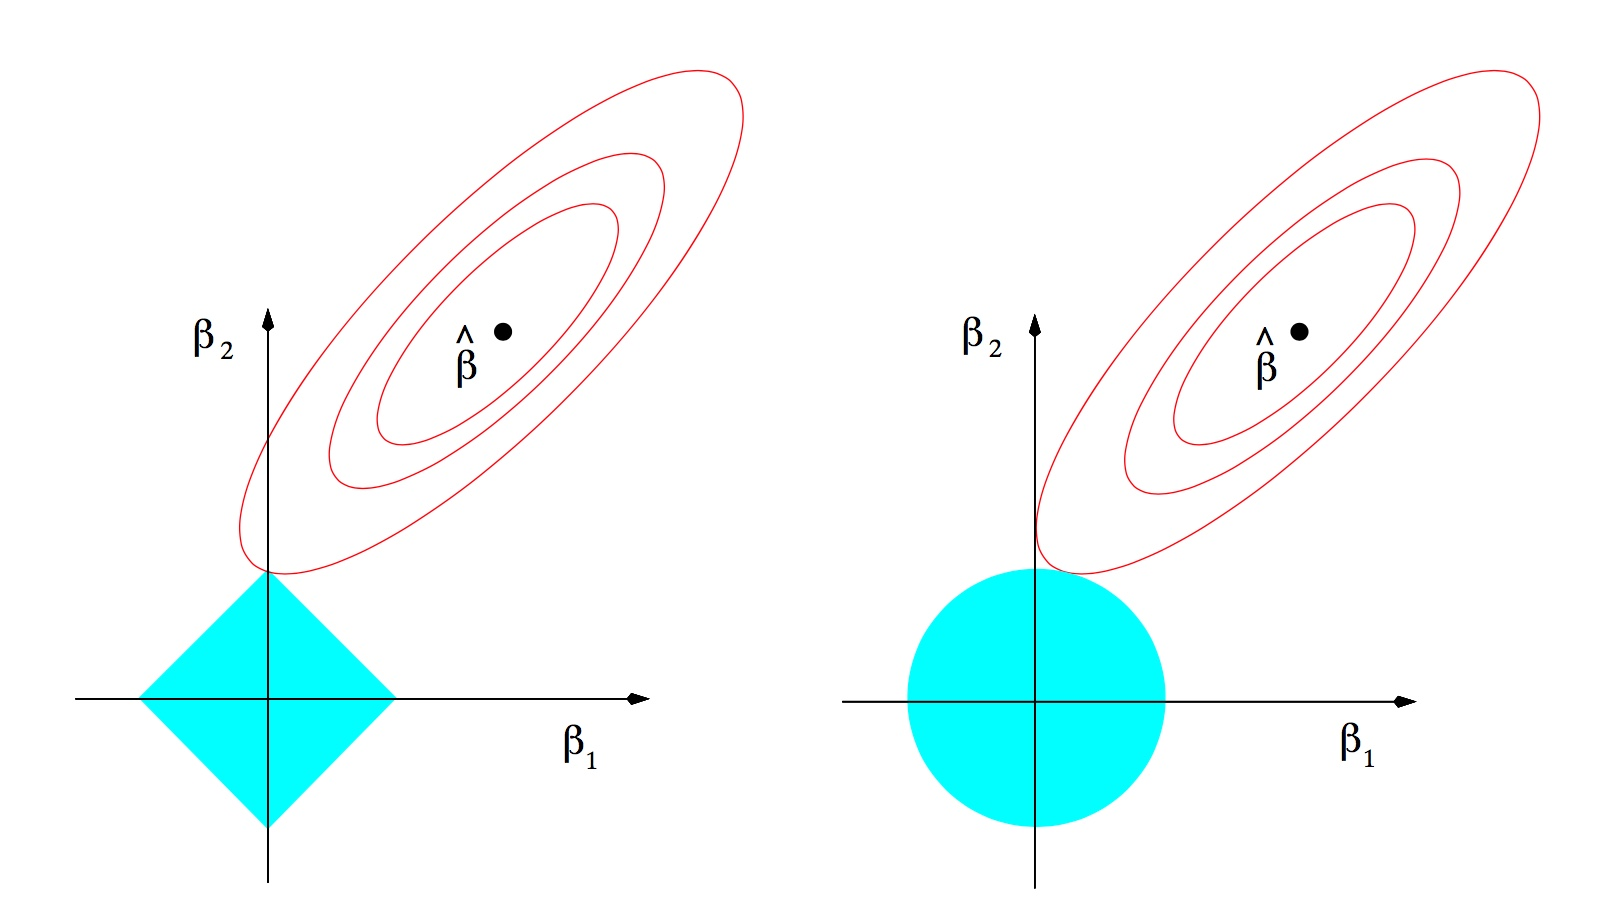
\includegraphics[width=5in]{l1_l2_balls.jpeg}
      \caption{The constrained optimization problems in $d=2$. Left: Lasso
        ($\ell_1$ ball). Right: Ridge ($\ell_2$ ball).
      Source: ESL}
    \end{figure}


\subsection{Orthogonal design}

Here is another way to understand why Lasso solutions are sparse.
Consider the case where all features are orthogonal, namely $XX^\Tr=I$. This is
in some sense the simplest setup for regression - we write $\V{y}$ as a linear
combination of {\bf orthonormal} vectors.
Statisticians call such $X$ an {\bf orthogonal design}.
\\~\\
 For $x\in\R$ and $\lambda\geq 0$ let us define two important functions
 $\R\to\R$: 
 \begin{itemize}
        \item ``soft threshold at $\lambda$''
          is the function $\eta^{soft}_\lambda:\R\to\R$ defined by
          \[
            \eta^{soft}_\lambda(x) = 
\begin{cases}
  x-\lambda \,\,& x\geq \lambda \\
  0 \,\,& \lambda > x > -\lambda \\
  x+\lambda \,\,& -\lambda\geq x
\end{cases}
          \]
        \item
          ``hard threshold at $\lambda$'' is the function 
          $ \eta^{hard}_\lambda:\R\to\R$ defined by
          \[
            \eta^{hard}_\lambda(x) = x\cdot \mathbf{1}_{|x|\geq \lambda}
            \]
      \end{itemize}

  ~\\
  Now, for $\lambda\geq 0$, let $\hat{\V{w}}^{LS}$, 
      $\hat{\V{w}}_\lambda^{ridge}$,
      $\hat{\V{w}}_\lambda^{lasso}$,
      $\hat{\V{w}}_\lambda^{subset}$
      denote the least squares (standard linear regression), Ridge, Lasso and
      Best Subset solutions, respectively.  
      \\~\\
      {\bf Claim.} 
      For a vector $\V{w}\in\R^d$ and a function $\eta:\R\to\R$ write 
      $\eta(\V{w})\in\R^d$ for the vector obtained by applying $\eta$ to each
      of the coordinates of $\V{w}$ separately.
      Assume orthogonal design. Then the Ridge, Lasso and Best
      subset solutions are given by 
      \begin{itemize}
        \item $\hat{\V{w}}_\lambda^{ridge} = \hat{\V{w}}^{LS} / (1+\lambda) $
        \item $\hat{\V{w}}_\lambda^{lasso} = \eta^{soft}_\lambda(\hat{\V{w}}^{LS})  $
        \item $\hat{\V{w}}_\lambda^{subset} = \eta^{hard}_{\sqrt{\lambda}}(\hat{\V{w}}^{LS})  $
      \end{itemize}
      (You will prove this in the recitation and homework.)
      \\~\\
      Namely, in this case, we can obtain the best subset, Lasso and Ridge
      solutions by applying {\bf univariate shrinkage functions} to each
      coordinate of $\hat{\V{w}}^{LS}$ separately. 
\\~\\
      Now observe (see figure) that in the orthogonal design case, 
      the best subset solution sets some weights to zero and leaves the rest
      untouched; the Lasso solution sets some weights to zero and ``shrinks''
      the rest a little; and the Ridge solution just multiplies by a scalar. So
      in the orthogonal design case we see how adding regularization 
      $\ell_0$ ``norm'' and $\ell_1$ norm induces sparse solutions, that get
      more and more sparse as $\lambda$ grows. A similar phenomenon, yet much
      more complicated, happens in the general case.
\begin{figure}[H]
      \centering
      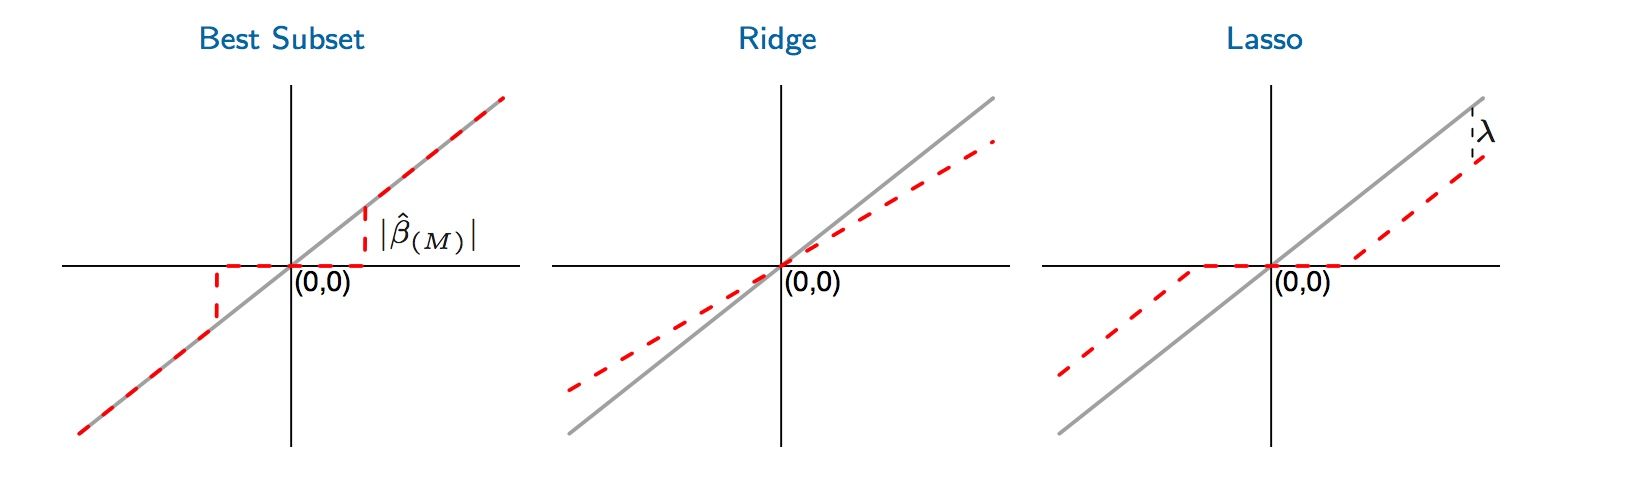
\includegraphics[width=6in]{orthogonal_design_shrink.jpeg}
      \caption{The constrained optimization problems in $d=2$. Left: Lasso
        ($\ell_1$ ball). Right: Ridge ($\ell_2$ ball).
      Source: ESL}
    \end{figure}




\section{$\ell_1$-regularized logistic regression}

We have seen a few different regression methods using regularization. To remind
us that regularization is a general principle, let's have a look at a
classification method using regularization. 
\\~\\
Recall that in logistic regression, our training sample 
is organized as regression matrix $X$ and a
label vector $\V{y}\in\left\{ 0,1 \right\}^m$.
\\~\\
If $m\sim d$ or even $d>m$ (not to mention the really high dimensional case
$d\gg m$), logistic regression will  suffer the same problems as linear
regression -  optimization will be numerically unstable; we can have large
coefficients of opposite signs for parallel feature vectors; interpretation will
be hard; and so on. All these problems are alleviated by adding a regularization
term. 
\\~\\
Recall that the logistic regression classifier finds the weight vector by solving
 \[
      \hat{\VV{w}} := 
      \argmax_{\VV{w}\in\reals^{d}}  
      \sum_{i=1}^m \left[ y_i (w_0+\innerr{\VV{x_i}}{\VV{w}}) - \log
      \left(1+e^{w_0+\innerr{\VV{x_i}}{\VV{w}}}\right) \right]\,,
    \]
    where (unlike the classification lecture)
    we did not include the intercept $w_0$ in the vector $\V{w}$, so
    $\V{w}\in\R^d$.
\\~\\
    So the fidelity term, which is minimized in the unregularized problem, is  
    \[
      \Fc_S(\V{w}) = 
       \sum_{i=1}^m \left[\log
      \left(1+e^{w_0\innerr{\VV{x_i}}{\VV{w}}}\right) 
-
        y_i (w_0+\innerr{\VV{x_i}}{\VV{w}})  \right]   \]
~\\
      While $\ell_1$-regularized linear regression has a fancy nickname (Lasso),
      $\ell_1$-regularized logistic regression does not have a nickname. 
      This learner simply adds the regularization term
      $\Rc(\V{w})=\norm{\V{w}}_1$ - just like the Lasso - to the fidelity term. 
      \\~\\
      So the $\ell_1$-regularized logistic regression classifier solves
      \[
        \text{argmin}_{\V{w}\in\R^d}
        \left[
        \sum_{i=1}^m \left[\log
      \left(1+e^{w_0+\innerr{\VV{x_i}}{\VV{w}}}\right) 
-
        y_i (w_0+\innerr{\VV{x_i}}{\VV{w}})  \right]  + \lambda\norm{\V{w}}_1\right] \]
      \\~\\
      This is a convex optimization problem, and fast 
      specialized solvers are
      available. $\ell_1$-regularized logistic regression is a great classifier
      for $\X=\R^d$ - it has low variance (as it is a linear classifier), we can
      control the bias-variance tradeoff by choosing $\lambda$; it is very
      (very!) interpretable, and so on.


\section{Practical considerations}

\subsection{Choosing lambda}

By now you're probably asking yourself how to choose $\lambda$, the
regularization parameter, based on the training sample alone. We'll address this
extensively in the next lecture.

\subsection{Intercept}

Notice that we never include the intercept $w_0$ in the regularization term. One
way to simplify everything would be to {\bf center} the rows of $X$, and then we
can disregard the intercept (see ESL exercise 3.5).

\subsection{Software implementation}

There are various software implementations for CART regression trees and random
forests for regression. There are various software implementations for best
subset selection (for small $d$).
For Ridge, Lasso and $\ell_1$ regularized logistic regression, we mention the
package 
{\tt glmnet} (with bindings to both {\tt python} and {\tt R}, which offers a correct, fast implementation solving the entire
regularization path. It also has other goodies such as cross-validation for
choosing $\lambda$ (which we will discuss in the next lecture), a method for
plotting the regularization path, combining $\ell_1$ and $\ell_2$
regularization terms, and more.





